\documentclass[a4paper,12pt]{article} 
\usepackage{amsmath}
\usepackage[retainorgcmds]{IEEEtrantools}
\usepackage{graphicx}
\usepackage{amsfonts}
\usepackage{amsthm}
\usepackage{centernot}
\usepackage{setspace}
\usepackage{mathtools}
\usepackage{amssymb}
\usepackage{bm}
\usepackage[mathscr]{euscript}
\usepackage{pictexwd,dcpic}
\usepackage{tikz}
\usepackage{tikz-cd}
\usepackage[margin=1in]{geometry}
\usepackage{breqn}
\newtheoremstyle{perfect}% name
  {}%         Space above, empty = `usual value'
  {}%         Space below
  {}% Body font
  {}%         Indent amount (empty = no indent, \parindent = para indent)
  {\bfseries}% Thm head font
  {.}%        Punctuation after thm head
  {\newline}% Space after thm head: \newline = linebreak
  {}%         Thm head spec
\theoremstyle{perfect}
\newtheorem{lem}{Lemma}
\newtheorem{thm}{Theorem}
\newtheorem{dfn}{Definition}
\newtheorem{exm}{Example}
\newtheorem{prop}{Proposition}
\newtheorem{crl}{Corollary}
\newtheorem{rem}{Reminder}
\newtheorem{prb}{Problem}
\newtheorem{exe}{Exercise}
\makeatletter
\newenvironment{cprb}[1]
  {\count@\c@prb
   \global\c@prb#1
    \global\advance\c@prb\m@ne
   \prb}
  {\endprb
   \global\c@prb\count@}
\makeatother
\makeatletter
\newenvironment{cexe}[1]
  {\count@\c@exe
   \global\c@exe#1
    \global\advance\c@exe\m@ne
   \exe}
  {\endexe
   \global\c@exe\count@}
\makeatother
\newcommand{\varline}{0}
\newcommand{\gen}[1]{\left< #1 \right>}
\newcommand{\ngen}[1]{\gen{\gen{#1}}}
\newcommand{\ov}[1]{\,\overline{#1}}
\DeclareMathOperator{\tor}{Tor}
\DeclareMathOperator{\aut}{Aut}
\DeclareMathOperator{\inn}{Inn}
\DeclareMathOperator{\im}{im}
\DeclareMathOperator{\imm}{Im}
\DeclareMathOperator{\ad}{ad}
\DeclareMathOperator{\Ad}{Ad}
\DeclareMathOperator{\Sp}{Sp}
\DeclareMathOperator{\SO}{SO}
\DeclareMathOperator{\SL}{SL}
\DeclareMathOperator{\SU}{SU}
\DeclareMathOperator{\GL}{GL}
\DeclareMathOperator{\PGL}{PGL}
\DeclareMathOperator{\re}{Re}
\DeclareMathOperator{\Hom}{Hom}
\DeclareMathOperator{\sym}{Sym}
\DeclareMathOperator{\ind}{Ind}
\DeclareMathOperator{\res}{Res}
\DeclareMathOperator{\sgn}{sgn}
\DeclareMathOperator{\End}{End}
\DeclareMathOperator{\colim}{colim}
\DeclareMathOperator{\coker}{coker}
\DeclareMathOperator{\Tr}{Tr}
\DeclareMathOperator{\intr}{int}
\DeclareMathOperator{\extr}{ext}
\DeclareMathOperator{\chr}{char}
\DeclareMathOperator{\supp}{supp}
\DeclareMathOperator{\hol}{Hol}
\DeclareMathOperator{\spec}{Spec}
\renewcommand{\Re}{\re}
\renewcommand{\Im}{\imm}
\newcommand{\eps}{\varepsilon}
\newcommand{\Mor}{\text{Mor}}
\newcommand{\cir}[1]{\mathrlap{\bigcirc}{\;#1}}
\newcommand{\Z}{\mathbb{Z}}
\newcommand{\Q}{\mathbb{Q}}
\newcommand{\R}{\mathbb{R}}
\newcommand{\C}{\mathbb{C}}
\newcommand{\F}{\mathbb{F}}
\newcommand{\N}{\mathbb{N}}
\newcommand{\lnorm}{\vartriangleleft}
\newcommand{\rnorm}{\vartriangleright}
\newcommand{\id}{\text{id}}
\newcommand{\dd}[1]{\mathrm{d}{#1}}
\newcommand{\p}[1]{\left( #1 \right)}
\newcommand{\parder}[2]{\frac{\partial #1}{\partial #2}}
\newcommand{\legendre}[2]{\left(\frac{#1}{#2}\right)}
\makeatletter
\renewcommand\part[1]{
\ifnum\pdfstrcmp{\varline}{1}=0
    \vspace{.10in}\textbf{\\#1)}
  \else
    \textbf{#1)}
  \fi\renewcommand{\varline}{1}}
\makeatother
\makeatletter
\newcommand{\tpmod}[1]{{\@displayfalse\pmod{#1}}}
\makeatother
\renewcommand{\restriction}{\mathord{\upharpoonright}}

\author{Konstantin Miagkov} 
\title{Lesson 6: Quadratic Equations V}
\begin{document} 
%\setstretch{1}
\maketitle

\begin{prb}
Let $f(x) = ax^2+bx+c$ be a quadratic function with $a > 0$, and set $h = -b/(2a)$. Show that the $f$ is decreasing from $-\infty$ to $h$ and increasing from $h$ to $+\infty$. In other words, show that for all $x,y$ such that $x < y < h$ we have $f(x) > f(y)$, and for all $x,y$ with $h < x < y$ we get $f(x) < f(y)$. What happens when $a < 0$? \textit{Hint: complete the square!}
\end{prb}

\begin{prb}
Find all values of $c$ for which the equation $x^2-4x+c = 0$ has two real roots whose sum of squares is 12.
\end{prb}

\begin{prb}
The picture below represents the graph of a quadratic equation $f$ with the $y$-axis erased. Assume that $f$ is monic ($a=1$), and the consecutive points on the $x$-axis are $1$ apart. Deduce the discriminant of $f$ from this picture alone.
\begin{center}
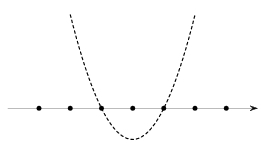
\includegraphics[scale=1.0]{parabola.jpg}
\end{center}
\end{prb}

\begin{prb}
Show that a quadratic equation $f$ with two distinct real roots $x_0, x_1$ is an even function if and only if $x_0 = -x_1$.
\end{prb}

\pagebreak

\begin{prb}
Three circles with the same radius $1$ are pairwise externally tangent to each other. If $A_1,A_2,A_3$ are the three tangency points, find the angles and side lengths of the triangle $\triangle A_1A_2A_3$.
\begin{center}
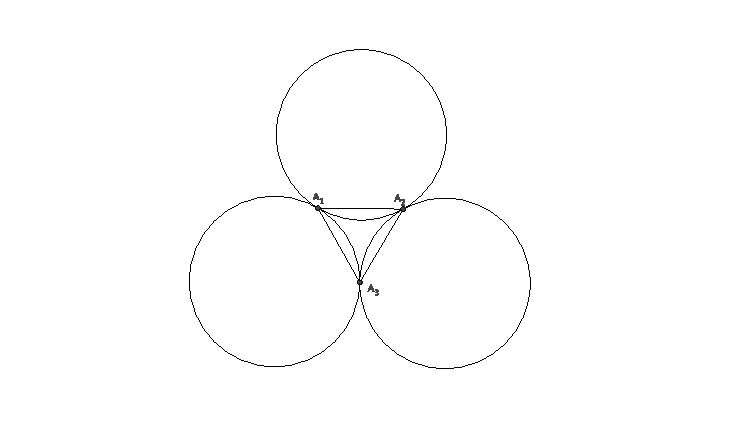
\includegraphics[scale=1.2]{three_circles.pdf}
\end{center}
\end{prb}

\begin{prb}
In a triangle $ABC$ we have $\angle ACB = 135^\circ$. Let $ABMN$ be a square lying to the opposite side of $C$ with respect to $AB$, and let $O$ be the intersection of its diagonals. If $AM = 12$, find $OC$.
\end{prb}




\end{document}